\documentclass[aspectratio=169]{beamer}
\usepackage[utf8]{inputenc}
\usepackage{hyperref}
\usepackage{amsmath,amsfonts,amsthm,bm}
\usepackage{color}
\usepackage{graphicx} % Allows including images
\usepackage{subcaption}
\usepackage{booktabs} % Allows the use of \toprule, \midrule and \bottomrule in tables
\usepackage{tikz}
%\usepackage{pgfplots}
\usepackage{adjustbox}
\usepackage{listings}
\usepackage{courier}
\usepackage[version=4]{mhchem}
\usepackage{array}

\lstset{ %
  basicstyle=\scriptsize\ttfamily, % fonts that are used for the code
  breakatwhitespace=false,         % sets if automatic breaks should only happen at whitespace
  %breaklines=true,                 % sets automatic line breaking
  %captionpos=b,                    % sets the caption-position to bottom
  commentstyle=\color{gray}\textit,    % comment style
  keepspaces=true,                 % keeps spaces in text, useful for keeping indentation of code (possibly needs columns=flexible)
  keywordstyle=\color{blue},       % keyword style
  language=Python,                 % the language of the code
  %otherkeywords={*,...},          % if you want to add more keywords to the set
  rulecolor=\color{black},         % if not set, the frame-color may be changed on line-breaks within not-black text (e.g. comments (green here))
  showspaces=false,                % show spaces everywhere adding particular underscores; it overrides 'showstringspaces'
  showstringspaces=false,          % underline spaces within strings only
  showtabs=false,                  % show tabs within strings adding particular underscores
  stringstyle=\color{red}, % string literal style
  tabsize=4,	                   % sets default tabsize to 2 spaces
  columns=fixed                    % Using fixed column width (for e.g. nice alignment)
}

\hypersetup{
    colorlinks=true,
    linkcolor=red,
    filecolor=magenta,      
    urlcolor=red,
}

\DeclareMathOperator*{\argmax}{argmax}
\DeclareMathOperator*{\argmin}{argmin}
\let \vec \mathbf

\newcommand{\classname}{NANO266}
\newcommand{\classyear}{Fall 2024}
\mode<presentation> {
    \usetheme{CambridgeUS}
    \setbeamertemplate{footline}[text line]{%
      \parbox{\linewidth}{\vspace*{-8pt}\classname\hfill\classyear\hfill\insertpagenumber}}

    %\setbeamertemplate{footline}[page number]
    \setbeamertemplate{navigation symbols}{}
}


\title[\classname Introduction to Quantum Mechanics]{\classname~- Quantum Mechanical Modeling of Materials and Nanostructures\\Introduction to Quantum Mechanics}

\author{Shyue Ping Ong}
\institute[UCSD]{University of California, San Diego\\
\medskip
}
\date{\classyear} % Date, can be changed to a custom date

\begin{document}


\begin{frame}
    \titlepage % Print the title page as the first slide
\end{frame}


\begin{frame}{Arguably the biggest scientific revolution in the 20th century with impact on the lives of people}
\begin{columns}
\column{0.8\textwidth}
\begin{tabular}{cl}
\small
1900 & Max Planck suggests quantization of radiation\\
1905 & Albert Einstein proposes light quanta that behaves like a particle\\
1913 & Bohr constructs a quantum theory of atomic structure\\
1924 & de Broglie proposes matter has wave-like properties\\
1925 & Pauli formulates exclusion principle\\
1926 & Schrodinger develops wave mechanics\\
1927 & Hsienberg formulates the uncertainty principle\\
1928 & Dirac combines QM with special relativity\\
& … and many more developments thereafter …
\end{tabular}
\column{0.2\textwidth}
\begin{figure}
    \centering
    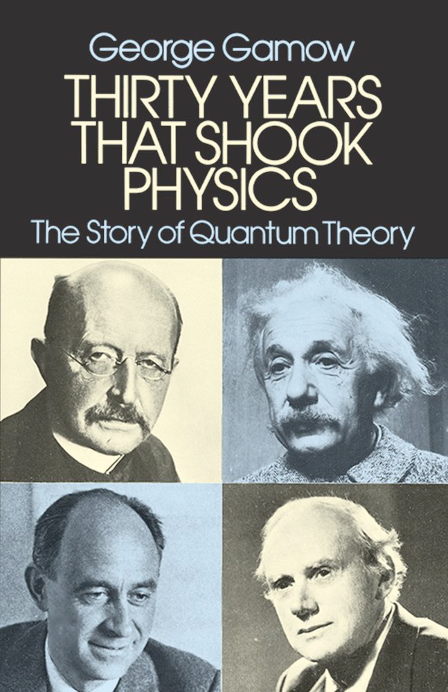
\includegraphics[width=\linewidth]{lectures/figures/30yearsthatshookphysics.png}
\end{figure}
\end{columns}
\end{frame}


\begin{frame}{First principles computational materials design}
\begin{columns}
    \column{0.5\textwidth}
\begin{equation*}
    \begin{aligned}
    \left[-\frac{\bar{h}^2}{2m}\nabla^2 + V(\vec{r})\right]\psi(\vec{r}) & =  E\psi(\vec{r}) \\
    & \downarrow  \\
    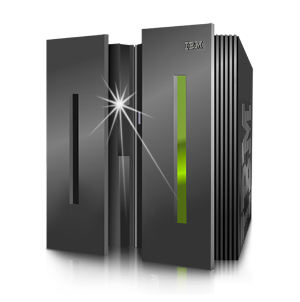
\includegraphics[width=0.35\textwidth]{lectures/figures/computer.png} & 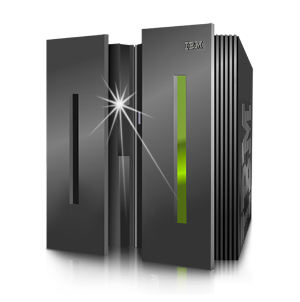
\includegraphics[width=0.35\textwidth]{lectures/figures/computer.png}  \\
    &\downarrow  \\
    & \mbox{\large{Materials Properties}}
    \end{aligned}
\end{equation*}
\column{0.5\textwidth}
\begin{itemize}
    \item Generally applicable to any chemistry.
    \item Inherently scalable through more computing.
\end{itemize}
\begin{figure}
    \centering
    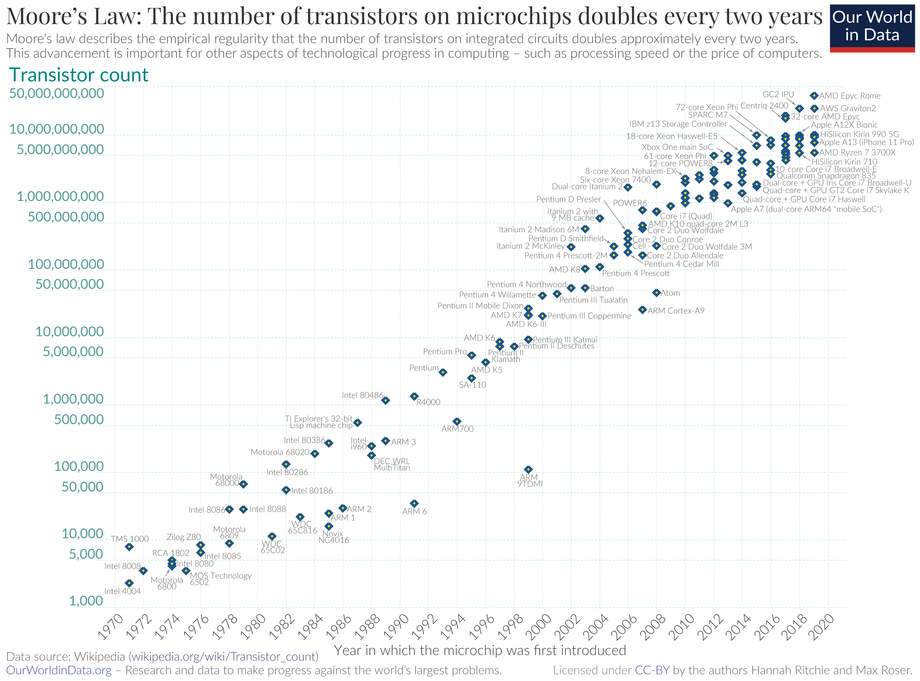
\includegraphics[width=0.7\linewidth]{lectures/figures/1_moores_law.png}
    \caption{Moore's law}
\end{figure}
\end{columns}

\end{frame}


\begin{frame}{Many properties can now be predicted with quantum mechanics}
\begin{figure}
    \centering
    \begin{subfigure}{0.2\textwidth}
        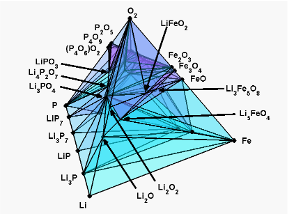
\includegraphics[width=\linewidth]{lectures/figures/1_phase_diagram.png}
    \caption{Phase stability\cite{ongLiFeO22008}}
    \end{subfigure}
    \begin{subfigure}{0.2\textwidth}
        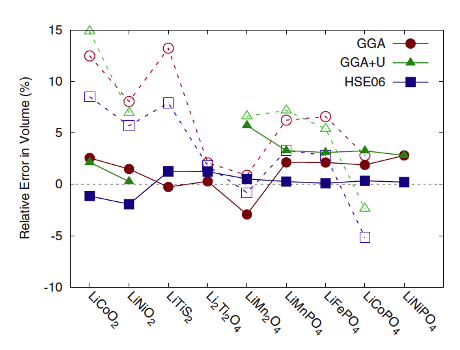
\includegraphics[width=\linewidth]{lectures/figures/1_Voltage.png}
    \caption{Voltages\cite{chevrierHybridDensityFunctional2010}}
    \end{subfigure}
    \begin{subfigure}{0.2\textwidth}
        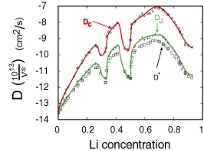
\includegraphics[width=\linewidth]{lectures/figures/1_Diffusivity.jpg}
    \caption{Diffusivity\cite{vandervenLithiumDiffusionLayered2000}}
    \end{subfigure}\\
    \begin{subfigure}{0.2\textwidth}
        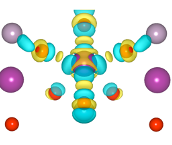
\includegraphics[width=\linewidth]{lectures/figures/1_polarons.png}
    \caption{Polarons\cite{ongComparisonSmallPolaron2011}}
    \end{subfigure}
        \begin{subfigure}{0.2\textwidth}
        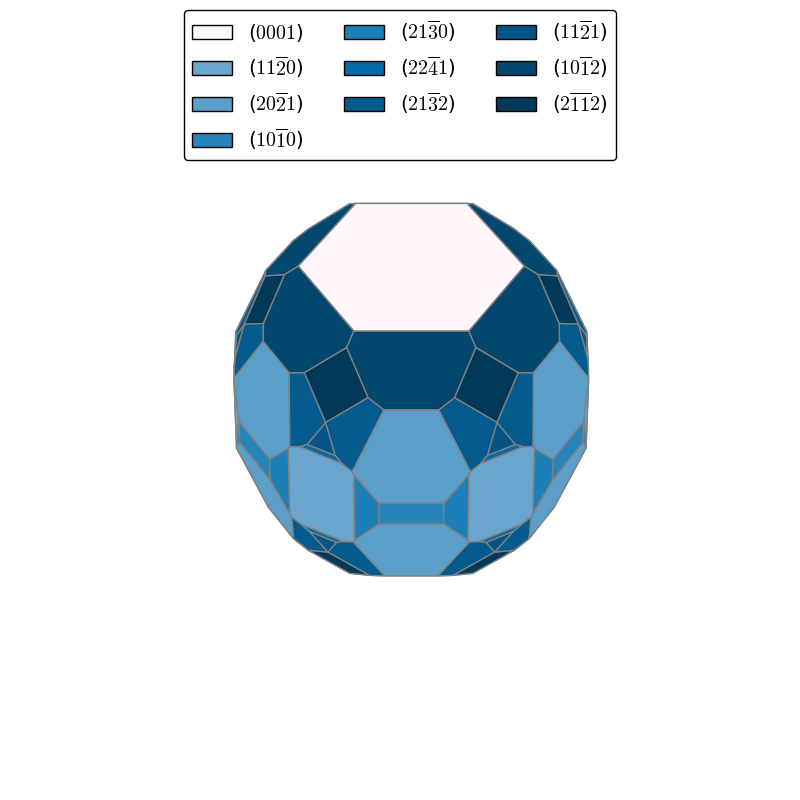
\includegraphics[width=\linewidth]{lectures/figures/1_surfaces.png}
    \caption{Surface energies\cite{tranSurfaceEnergiesElemental2016}}
    \end{subfigure}
\end{figure}

\end{frame}


\begin{frame}{First principles calculations are now an essential materials science tool}
\begin{figure}
    \centering
    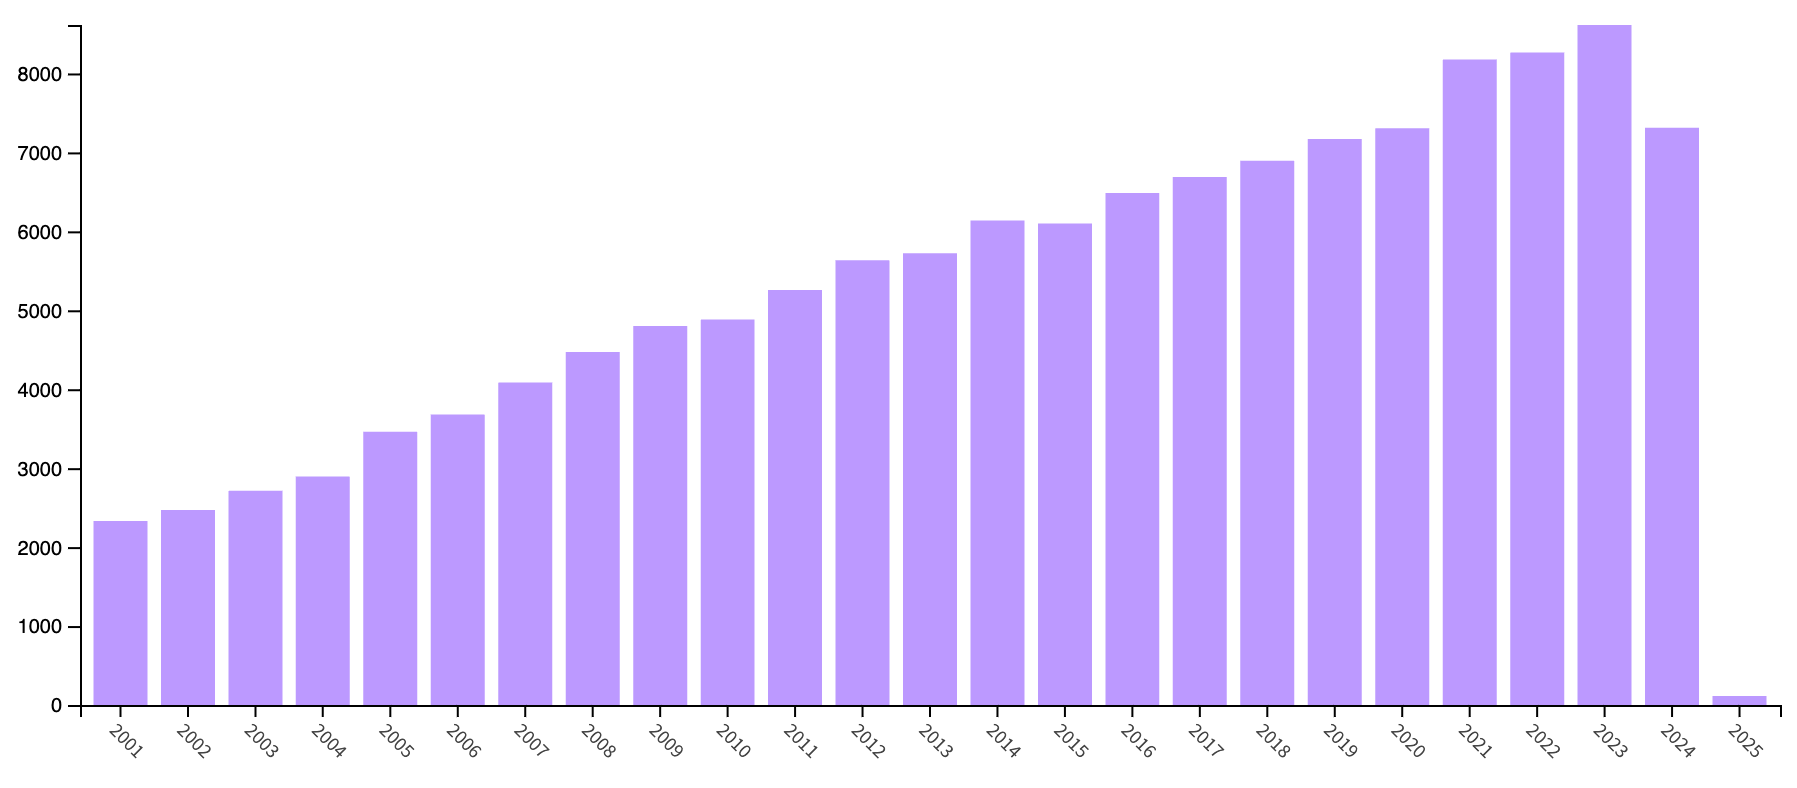
\includegraphics[width=0.8\linewidth]{lectures/figures/1_Papers_per_year.png}
    \caption{Published articles per year with "DFT", "Ab initio", "First Principles" in title. Source: Web of Science. Note: This excludes papers that do not mention these terms in the title but nonetheless utilize such calculations in the work.}
\end{figure}
\end{frame}


\begin{frame}{The Schr\"odinger Equation}

\begin{equation}
\large
    -i\bar{h}\frac{d}{dt}\psi(\vec{r},t)=\left[-\frac{\bar{h}^2}{2m}\nabla^2 + V(\vec{r},t)\right]\psi(\vec{r}, t) = E\psi(\vec{r},t)
\end{equation}
The underlying physical laws necessary for the mathematical theory of a \textbf{large part of physics and the whole of chemistry} are thus completely known, and the difficulty is only that the exact application of these laws leads to equations much too complicated to be soluble.\\
- Paul Dirac, 1929

\end{frame}


\begin{frame}{Tradeoff Trinity}
\begin{figure}
    \centering
    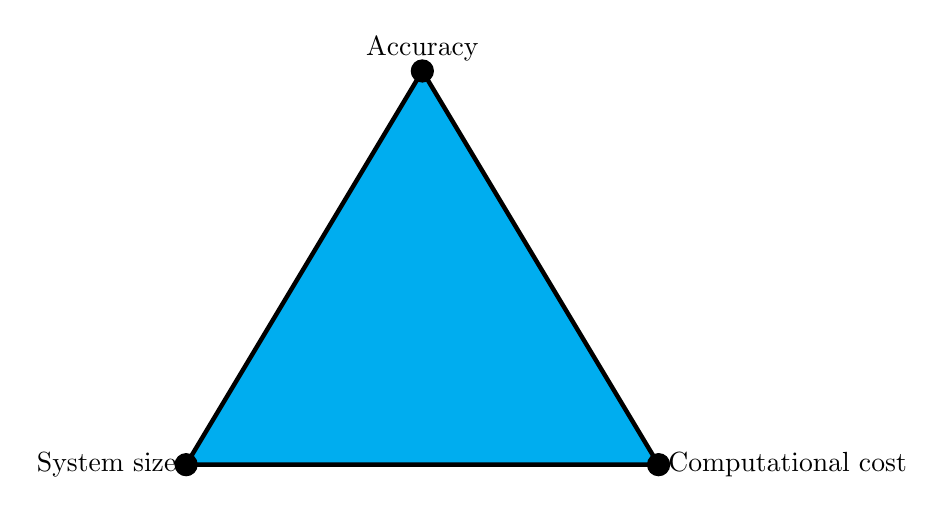
\begin{tikzpicture}
    \filldraw[color=black, fill=cyan, ultra thick] (4,0) -- (10,0) -- (7,5) -- cycle;
    \filldraw[black] (4,0) circle (4pt) node[anchor=east]{System size};
    \filldraw[black] (10,0) circle (4pt) node[anchor=west]{Computational cost};
    \filldraw[black] (7,5) circle (4pt) node[anchor=south]{Accuracy};
    \end{tikzpicture}
    \caption{Choose two (sometimes you only get one)}
\end{figure}

\end{frame}


\begin{frame}{Stationary Schr\"odinger Equation}

If the external potential has no time dependence, we can write the wave function as a separable function:
\begin{equation*}
\psi(\vec{r},t)=\phi(\vec{r})f(t)
\end{equation*}
And the Schrödinger Equation can be decomposed to:

\begin{eqnarray*}
    -i\bar{h}\frac{d}{dt}f(t) & = & Ef(t) \implies f(t) = e^{-i\frac{E}{\bar{h}}t}\\
    \left[-\frac{\bar{h}^2}{2m}\nabla^2 + V(\vec{r})\right]\phi(\vec{r}) & = & E\phi(\vec{r}) - \mbox{\textcolor{red}{Stationary Schr\"odinger Equation}}
\end{eqnarray*}

\end{frame}


\begin{frame}{Stationary Schr\"odinger Equation}
\begin{eqnarray*}
    H\phi(\vec{r}) = E\phi(\vec{r}) 
\end{eqnarray*}
where

\begin{eqnarray*}
    H = -\sum_i \frac{\bar{h}^2}{2m_e}\nabla_i^2
    -\sum_k \frac{\bar{h}^2}{2m_k}\nabla_k^2
    -\sum_i\sum_k \frac{e^2Z_k}{r_{ik}}
    +\sum_i\sum_j \frac{e^2}{r_{ij}}
    +\sum_k\sum_l \frac{e^2Z_kZ_l}{r_{kl}}
\end{eqnarray*}
    KE of electrons: $-\sum_i \frac{\bar{h}^2}{2m_e}\nabla_i^2$, KE of nuclei: $-\sum_k \frac{\bar{h}^2}{2m_k}\nabla_k^2$\\
    Coulombic attraction between nuclei and electrons : $-\sum_i\sum_k \frac{e^2Z_k}{r_{ik}}$\\
    Coulombic repulsion between electrons and between nuclei:$\sum_i\sum_j \frac{e^2}{r_{ij}}$, $\sum_k\sum_l \frac{e^2Z_kZ_l}{r_{kl}}$

\end{frame}

\begin{frame}{Two broad approaches to solving the Schr\"odinger equation}
\begin{columns}
    \column{0.5\textwidth}
    \begin{figure}
        \centering
        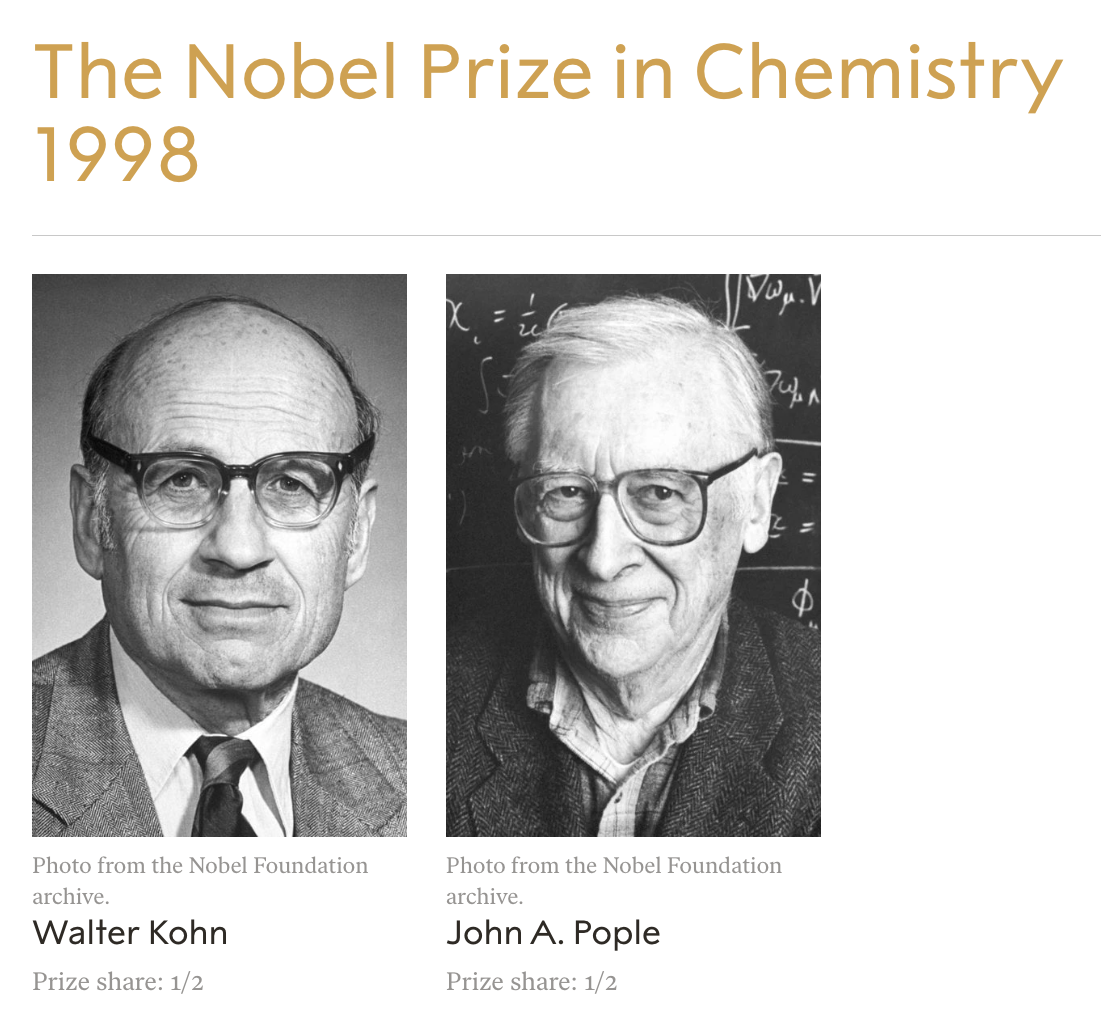
\includegraphics[width=0.9\linewidth]{lectures/figures/1_nobelprizes.png}
    \end{figure}
    \column{0.5\textwidth}
    The Nobel Prize in Chemistry 1998 was divided equally between Walter Kohn ``for his development of the density-functional theory'' and John A. Pople ``for his development of computational methods in quantum chemistry''.
    
\end{columns}
    
\end{frame}

\begin{frame}{Two broad approaches to solving the Schr\"odinger equation}

\begin{table}[]
    \centering
    \begin{tabular}{p{7cm}|p{7cm}}
        \textbf{Variational Approach} & \textbf{Density Functional Theory (DFT)}  \\
        \hline\hline
        Expand wave function as a linear combination of basis functions & In principle exact\\
        \hline
        Results in matrix eigenvalue problem & In practice, many approximate schemes\\
        \hline
        Clear path to more accurate answers (increase no. of basis functions, number of clusters / configurations) & Computational cost comparatively low\\
        \hline
        Favored by quantum chemists & Favored by solid-state community\\
    \end{tabular}
\end{table}
    
\end{frame}

\begin{frame}{Solving the Schr\"odinger equation}

In general, there is a complete set of eigenfunctions $\psi_i$ with corresponding eigenvalues $E_i$. Without loss of generality, let us assume that the wave functions are orthonormal:
\begin{equation*}
    \int \psi_i^*\psi_j d\vec{r} = \delta_{ij}
\end{equation*}
    Hence,
    \begin{equation*}
    \int \psi_i^*H\psi_j d\vec{r} = \int \psi_i^*E\psi_j d\vec{r}=E\delta_{ij}
\end{equation*}
\end{frame}


\begin{frame}{The Variational Principle}

Let us define a guess wave function that is a linear combination of the real wave functions
\begin{equation*}
    \phi = \sum_i c_i\psi_i
\end{equation*}
    Hence,
    \begin{eqnarray*}
    \int |\phi|^2 d\vec{r} & = & \sum_i c_i^2\\
    \int \phi^* H \phi d\vec{r} & = & \sum_i c_i^2E_i
    \end{eqnarray*}


Let us define the lowest $E_i$ as the ground state $E_0$
\begin{equation*}
    \int \phi^* H \phi d\vec{r} - E_0 \int |\phi|^2 d\vec{r} =  \sum_i c_i^2(E_i-E_0)
\end{equation*}
\end{frame}

\begin{frame}{The Variational Principle}

Since the RHS is always positive,

    \begin{eqnarray*}
    \int \phi^* H \phi d\vec{r} - E_0 \int |\phi|^2 d\vec{r} & \geq & 0\\
    \frac{\int \phi^* H \phi d\vec{r}}{\int |\phi|^2 d\vec{r}} \geq E_0
    \end{eqnarray*}
\begin{alertblock}{Key takeaway}
We can judge the quality of a guess wave functions by the energy – \textbf{the lower the energy, the better}. We may also use any arbitrary basis set to expand the guess wave function.
\end{alertblock}
\end{frame}



\begin{frame}[allowframebreaks]{Bibliography}
    \bibliographystyle{unsrt}
    \bibliography{refs}
\end{frame}



\begin{frame}
    \Huge{\centerline{The End}}
\end{frame}

\end{document}

